\documentclass[a4paper,11pt]{article}
\usepackage{amssymb}
\usepackage[polish]{babel}
\usepackage[utf8]{inputenc}
\usepackage[T1]{fontenc}
\usepackage{array}
\usepackage{graphicx}
\usepackage{anysize}
\usepackage{enumerate}
\usepackage{times}
\usepackage{geometry}
\usepackage{amsthm}
\usepackage{pgfplots}
\usepackage{sidecap}
\usepackage{wrapfig}
\usepackage[format=hang,font=small,labelfont=bf]{caption}


\usepackage[intlimits]{amsmath}
\marginsize{3cm}{3cm}{1.5cm}{1.5cm}
\sloppy

\begin{document}
\begin{table}[ht]
\centering
\hspace*{-1cm}
\begin{tabular}{lllllll}
\cline{1-6}
\multicolumn{1}{|c|}{\begin{tabular}[c]{@{}c@{}}EAIiIB\\ Informatyka\end{tabular}}              & \multicolumn{2}{l|}{\begin{tabular}[c]{@{}l@{}}Ewa Stachów\\ Weronika Olcha\end{tabular}}                                                                                                & \multicolumn{1}{c|}{\begin{tabular}[c]{@{}c@{}}Rok\\ II\end{tabular}}          & \multicolumn{1}{c|}{\begin{tabular}[c]{@{}c@{}}Grupa\\ 3\end{tabular}}            & \multicolumn{1}{c|}{\begin{tabular}[c]{@{}c@{}}Zespół\\ 6\end{tabular}}      &  \\ \cline{1-6}
\multicolumn{1}{|c|}{\begin{tabular}[c]{@{}c@{}}Pracownia\\ FIZYCZNA\\ WFiIS AGH\end{tabular}} & \multicolumn{4}{l|}{\begin{tabular}[c]{@{}l@{}}Temat:\\ \textbf{\textit{Wahadło fizyczne}} \end{tabular}}                                                                                                                                                                                                                                            & \multicolumn{1}{c|}{\begin{tabular}[c]{@{}c@{}}Nr ćwiczenia:\\ 1\end{tabular}} &  \\ \cline{1-6}
\multicolumn{1}{|l|}{\begin{tabular}[c]{@{}c@{}}Data wykonania:\\ 14.10.2016\end{tabular}}      & \multicolumn{1}{c|}{\begin{tabular}[c]{@{}c@{}}Data oddania:\\ 19.10.2016\end{tabular}} & \multicolumn{1}{l|}{\begin{tabular}[c]{@{}l@{}}Zwrot do poprawki:\\ \phantom{data poprawki}\end{tabular}} & \multicolumn{1}{l|}{\begin{tabular}[c]{@{}l@{}}Data oddania:\\  \phantom{data oddania}\end{tabular}} & \multicolumn{1}{l|}{\begin{tabular}[c]{@{}l@{}}Data zaliczenia:\\  \phantom{data zaliczenia}\end{tabular}} & \multicolumn{1}{l|}{\begin{tabular}[c]{@{}l@{}}OCENA:\\ \phantom{ocena}\end{tabular}}       &  \\ \cline{1-6}
 
\end{tabular}
\end{table}

\begin{center}
\begin{LARGE}
\textbf{Ćwiczenie nr 1: Wahadło fizyczne}
\end{LARGE}
\end{center}



\section{Cel ćwiczenia}
Opis ruchu drgającego, a w szczególności drgań wahadła fizycznego. Wyznaczenie momentów bezwładności brył sztywnych.

\section{Wstęp teoretyczny}
Moment bezwładności punktu materialnego o masie $m$ obracającego się wokół osi $O$ w odległości $r$ definiujemy jako:
$$I=mr^{2}$$
Bryłę sztywną można traktować jako ciągły zbiór punktów materialnych o różnych odległościach od osi obrotu. Wobec powyższego moment bezwładności wyraża się następująco:
$$I=\int r^{2}dm$$
Wahadło fizyczne jest to bryła sztywna o masie $m$ zawieszona w punkcie $O$ różnym od środka ciężkości. Wahadło odchylone od pionu o kąt $\theta$, a następnie puszczone swobodnie będzie wykonywać pod wpływem momentu siły ciężkości drgania zwane ruchem wahadłowym. Moment tej siły dla wychylenia $\theta$ jest równy $mgasin\theta$. Ruch ten opisuje II zasada dynamiki dla ruchu obrotowego, zgodnie z którą iloczyn momentu bezwładności $I$  i przyspieszenia kątowego $\varepsilon$ jest równy działającemu momentowi siły, czyli:
$$ \varepsilon = \frac{d^{2}\theta}{dt^{2}} \Rightarrow I_{o}\displaystyle \frac{d^{2}\theta}{dt^{2}}=-mga\sin\theta$$
Siła $mgsin\theta$ jest zawsze skierowana przeciwnie do kierunku wychylenia -- stąd znak minus we wzorze.
Jeżeli rozpatrujemy ruch dla małych kątów wychylenia, to sinus kąta można zastąpić samym kątem w mierze łukowej, ponieważ $sin\theta \approx \theta$. Zatem powyższe równanie przyjmuje postać: 
$$\frac{d^{2}\theta}{dt^{2}} + \dfrac{mga\theta}{I_{o}}=0,$$
jest to równanie ruchu harmonicznego z okresem:
$$T=2\pi\sqrt{\frac{I_{o}}{mga}}$$
\textbf{Twierdzenie Steinera} mówi, że jeśli znamy moment bezwładności $I_{S}$ danego ciała względem pewnej osi przechodzącej przez środek masy tego ciała, to aby obliczyć moment bezwładności $I_{0}$ względem dowolnej innej osi równoległej do niej, należy do momentu $I_{S}$ dodać iloczyn masy ciała i kwadratu odległości $a$ między tymi osiami:
$$I_{0}=I_{S}+ma^{2}$$
\section{Układ pomiarowy}

\begin{itemize}
\item Statyw, na którym zawiesza się badaną bryłę
\item Badane bryły: pręt, pierścień
\item Metalowy przymiar milimetrowy
\item Suwmiarka
\item Waga elektroniczna
\item Sekundomierz
\end{itemize}

\begin{figure}[ht]
\centering
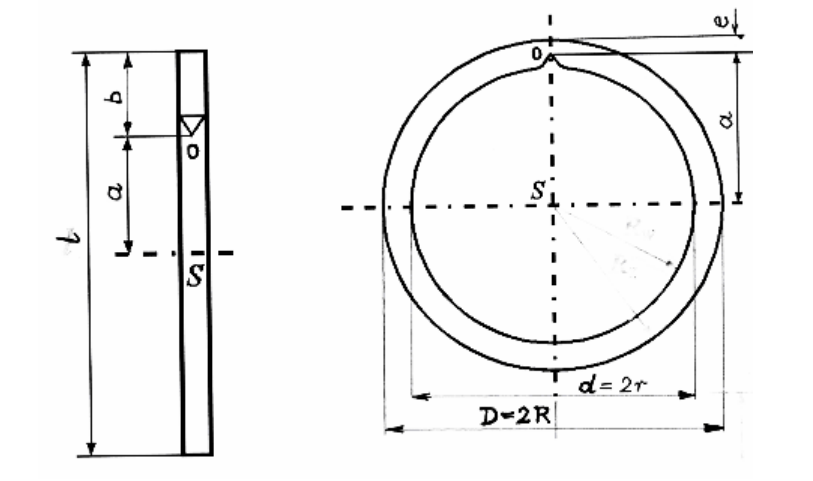
\includegraphics[width=0.7\linewidth]{./schemat}
\caption{Pręt i pierścień używane w ćwiczeniu.}
\end{figure}

\section{Wykonanie ćwiczenia}
Na początku ustalamy masę oraz określamy długości pręta i pierścienia, tak jak pokazano na Rysunku 1 (małe długości mierzymy suwmiarką). Umieszczamy pręt na statywie, wprowadzamy go w ruch drgający o amplitudzie
nieprzekraczającej trzech stopni i mierzymy czas trzydziestu drgań. Pomiar ten powtarzamy dziesięciokrotnie. Analogicznie postępujemy z pierścieniem.

 
\section{Opracowanie wyników pomiarów}

\begin{table}[ht]

\centering
\setlength{\extrarowheight}{2pt}
\caption{\textbf{Pomiar masy i długości pręta.}}
\begin{tabular}{| @{\hspace{8mm}}c @{\hspace{8mm}}| @{\hspace{8mm}}c @{\hspace{8mm}}|@{\hspace{8mm}} c@{\hspace{8mm}}|}
\hline
 & wartość & niepewność  \\ \hline
$m[g]$ & 663 & 0,1 \\ \hline
$l[mm]$ & 750 & 1 \\ \hline
$b[mm]$ & 100 & 1 \\ \hline
$a[mm]$ & 275 & 1 \\ \hline

\end{tabular}
\end{table}

\begin{table}[ht]
\centering
\setlength{\extrarowheight}{2pt}
\caption{\textbf{Pomiar masy i długości pierścienia.}}
\begin{tabular}{| @{\hspace{8mm}}c @{\hspace{8mm}}| @{\hspace{8mm}}c @{\hspace{8mm}}|@{\hspace{8mm}} c@{\hspace{8mm}}|}
\hline
 & wartość & niepewność  \\ \hline
$m[g]$ & 1360 & 0,1 \\ \hline
$D_{W}[mm]$ & 255,6 & 0,1 \\ \hline
$D_{Z}[mm]$ & 280,4 & 0,1 \\ \hline
$R_{W}[mm]$ & 127,8 & 0,1 \\ \hline
$R_{Z}[mm]$ & 140,2 & 0,1 \\ \hline
$e[mm]$ & 7,6 & 0,1 \\ \hline
$a[mm]$ & 132,6 & 0,1 \\ \hline

\end{tabular}
\end{table}

\begin{table}[ht]
\vspace*{0.5 cm}
\centering
\setlength{\extrarowheight}{2pt}
\caption{\textbf{Pomiar okresu drgań dla pręta.}}
\begin{tabular}{|c|c|c|c|}
\hline
Lp. & liczba okresów $k$ & czas $t$ dla $k$ okresów w [$s$] & okres $T_{i}=t/k$ w [$s$] \\ \hline
1 & 20 & 26,47 & 1,3235\\ \hline
2 & 20 & 26,84 & 1,342\\ \hline
3 & 20 & 26,68 & 1,334\\ \hline
4 & 20 & 26,69 & 1,3345\\ \hline
5 & 20 & 26,78 & 1,339\\ \hline
6 & 20 & 26,75 & 1,3375\\ \hline
7 & 20 & 26,75 & 1,3375\\ \hline
8 & 20 & 26,87 & 1,3435\\ \hline
9 & 20 & 26,54 & 1,327\\ \hline
10 & 20 & 26,78 & 1,339\\ \hline
\multicolumn{4}{|c|}{Wartość średnia okresu: $\overline{T}= 1,33575$} \\ \hline
\multicolumn{4}{|c|}{Niepewność: $u(T)\approx 0,0020$} \\ \hline
\end{tabular}
\end{table}

\begin{table}[!ht]
\vspace*{0.5 cm}
\centering
\setlength{\extrarowheight}{2pt}
\caption{\textbf{Pomiar okresu drgań dla pierścienia.}}
\begin{tabular}{|c|c|c|c|}
\hline
Lp. & liczba okresów $k$ & czas $t$ dla $k$ okresów w [$s$] & okres $T_{i}=t/k$ w [$s$] \\ \hline
1 & 20 & 20,72 & 1,036\\ \hline
2 & 20 & 20,79 & 1,0395\\ \hline
3 & 20 & 20,75 & 1,0375\\ \hline
4 & 20 & 20,72 & 1,036\\ \hline
5 & 20 & 20,69 & 1,0345\\ \hline
6 & 20 & 20,71 & 1,0355\\ \hline
7 & 20 & 20,69 & 1,0345\\ \hline
8 & 20 & 20,69 & 1,0345\\ \hline
9 & 20 & 20,62 & 1,031\\ \hline
10 & 20 & 20,82 & 1,041\\ \hline
\multicolumn{4}{|c|}{Wartość średnia okresu: $\overline{T}= 1,036s$} \\ \hline
\multicolumn{4}{|c|}{Niepewność: $u(T)\approx 0,00089s$} \\ \hline
\end{tabular}
\end{table}
$$$$
\subsection{Moment bezwładności $I_{0}$ względem rzeczywistej osi obrotu korzystając z~wzoru na okres drgań}
Wzór na okres drgań wyraża się wzorem:
$$T=2\pi\sqrt{\dfrac{I_{0}}{mga}}$$
Przekształcając odpowiednio powyższe równanie otrzymujemy wzór na moment bezwładności:
$$I_{0}=\dfrac{mgaT^{2}}{4\pi^{2}},$$
gdzie $m$ -- masa bryły, $g$ -- przyspieszenie ziemskie, $T$ -- okres drgań, $a$ -- odległość środka masy od osi obrotu.
$$$$
\textbf{Momement bezdładności $I_{0}$ dla pręta:}
$$I_{0} = \dfrac{0,663kg\cdot 9,811\dfrac{m}{s^{2}}\cdot 0,275m \cdot (1,33575s)^{2}}{4\pi^{2}}\approx ~0,08084 kg \cdot m^{2}$$
\textbf{Momement bezdładności $I_{0}$ dla pierścienia:}
$$I_{0} = \dfrac{1,36kg\cdot 9,811\dfrac{m}{s^{2}}\cdot 0,1326m \cdot (1,036s)^{2}}{4\pi^{2}}\approx 0,048096~ kg \cdot m^{2}$$

\subsection{Moment bezwładności $I_{S}$ względem osi przechodzącej przez środek masy korzystając z twierdzenia Steinera}
Twierdzenie Steinera stosuje się do obliczania momentu bezwładności bryły względem osi przesuniętej równolegle o długość $a$, gdzie $I_{S}$ to moment bezwładności względem osi przechodzącej przez środek masy bryły.
$$I_{0}=I_{S}+ma^{2}$$
$$I_{S}=I_{0}-ma^{2}$$
\textbf{Momement bezdładności $I_{S}$ dla pręta:
}$$I_{S} =0,080836 kg \cdot m^{2} - 0,663kg\cdot (0,275m)^{2}\approx 0,03070~kg \cdot m^{2}$$
\textbf{Momement bezdładności $I_{S}$ dla pierścienia:
}$$I_{S} = 0,048096 kg \cdot m^{2} - 1,36kg\cdot (0,1326m)^{2}\approx 0,02418~kg \cdot m^{2}$$

\subsection{Moment bezwładności względem osi przechodzącej przez środek masy $I_{S}^{(geom)}$ na podstawie masy i wymiarów geometrycznych}
Moment bezwładności większości regularnych brył można zapisać w postaci: 
$$I_{S}^{(geom)} = k \cdot m \cdot l,$$ 
gdzie $m$ -- masa bryły, $l$ -- charakterystyczny wymiar bryły (np. długość, promień), $k$ -- bezwymiarowy współczynnik
zależny tylko od kształtu bryły i wyboru charakterystycznego wymiaru (np. promień czy średnica), a niezależny od wielkości bryły.
$$$$
\textbf{Momement bezdładności $I_{S}^{(geom)}$ dla pręta:
}$$I_{S}^{(geom)} = \dfrac{1}{12}ml^{2}$$
$$I_{S}^{(geom)} = \dfrac{1}{12}\cdot 0,663kg\cdot (0,75m)^{2}\approx 0,031078kg \cdot m^{2}$$
\textbf{Momement bezdładności $I_{S}^{(geom)}$ dla pierścienia:
}$$I_{S}^{(geom)} = \dfrac{1}{12}m(R^{2}+r^{2})$$
$$I_{S}^{(geom)} = \dfrac{1}{12}\cdot 1,36kg\cdot ((0,1402m)^{2}+(0,1278m)^{2})\approx 0,024472kg \cdot m^{2}$$


\subsection{Niepewności mierzonych wielkości}
\subsubsection{Niepewność pomiaru okresu -- niepewność typu A}
Wzór na niepewność pomiaru $u(T)$:
$$u(T)=\displaystyle \frac{\sqrt{\frac{\sum(T_{i}-\overline{T})^{2}}{n-1}}}{\sqrt{n}}=\displaystyle \sqrt{\frac{\sum(T_{i}-\overline{T})^{2}}{n(n-1)}},$$
gdzie $n$ -- liczba pomiarów, $\overline{T}=\frac{1}{n}\sum T_{\mathrm{i}}$ -- średni czas trwania okresu.
$$$$
\textbf{Niepewność pomiaru okresu dla pręta:}
$$\overline{T}=1,33575s$$ 
$$u(T)=\displaystyle \sqrt{\frac{(1,3235s-1,33575s)^{2}+\cdots +(1,339s-1,33575s)^{2}}{10(10-1)}}\approx 0,0020s$$
\textbf{Niepewność pomiaru okresu dla pierścienia:}
$$\overline{T}=1,036s$$ 
$$u(T)=\displaystyle \sqrt{\frac{(1,036s-1,036s)^{2}+\cdots +(1,041s-1,036s)^{2}}{10(10-1)}} \approx 0,00089s$$
\subsubsection{Niepewność pomiaru masy}
Do określenia masy pręta i pierścienia posłużyła nam waga cyfrowa o dokładności $0,001kg$, więc $u(m)=1g$.
\subsubsection{Niepewność pomiaru wymiarów geometrycznych}
W pomiarze pręta przyjmujemy niepewność równą działce elementarnej linijki $u(l)=1mm$, $u(a)=1mm$, $u(b)=1mm$. Wszystkie wartości długości związanych z pierścieniem były mierzone za pomocą suwmiarki, której dokładność wynosiła $0,1mm$, zatem $u(D_{W})=0,1mm$, $u(D_{Z})=0,1mm$, $u(R_{W})=0,1mm$, $u(R_{Z})=0,1mm$, $u(e)=0,1mm$, $u(a)=0,1mm$.
\subsection{Niepewność złożona momentu bezwładności $I_{0}$}
Wzór z którego korzystamy:
$$\frac{u(I_o)}{I_0}=\sqrt{\left (\frac{u(m)}{m}\right ) ^2+\left ( \frac{u(a)}{a}\right )^2+\left (2 \frac{u(T)}{T}\right )^2}$$
\textbf{Niepewność złożona momentu bezwładności $I_{0}$ dla pręta:}
$$
\frac{u(I_o)}{I_0}=\sqrt{\left(\frac{0,001}{0,663}\right) ^2+\left( \frac{0,001}{0,275}\right)^2+\left(2 \frac{0,0020}{1,33575}\right)^2} \approx 0,0049
$$
$$u(I_0)\approx 0,00040~kg\cdot m^2$$
\textbf{Niepewność złożona momentu bezwładności $I_{0}$ dla pierścienia:}
$$
\frac{u(I_o)}{I_0}=\sqrt{\left(\frac{0,001}{1,36}\right) ^2+\left( \frac{0,0001}{0,1326}\right)^2+\left(2 \frac{0,00089}{1,036}\right)^2} \approx 0,0020
$$
$$u(I_0)\approx 0,000097~kg\cdot m^2$$
\subsection{Niepewność złożona momentu bezwładności $I_{S}$}
Wzór z którego korzystamy:
$$u(I_s)=\sqrt{\left( u(I_0)\right)^2+\left(a^2u(m) \right)^2+\left( -2amu(m)\right)^2}$$
\textbf{Niepewność złożona momentu bezwładności $I_{S}$ dla pręta:}
$$u(I_s)=\sqrt{\left( 0,00040\right)^2+\left(0,275^2\cdot 0,001 \right)^2+\left( -2\cdot 0,275\cdot 0,663\cdot 0,001\right)^2}~kg\cdot m^2$$
$$u(I_s)\approx 0,00055~kg\cdot m^2$$
\textbf{Niepewność złożona momentu bezwładności $I_{S}$ dla pierścienia:}
$$u(I_s)=\sqrt{\left( 0,000097\right)^2+\left(0,1326^2\cdot 0,001 \right)^2+\left( -2\cdot 0,1326\cdot 1,36\cdot 0,001\right)^2}~kg\cdot m^2$$
$$u(I_s)\approx 0,00037~kg\cdot m^2$$

\subsection{Niepewność $u_{c}(I_{S}^{(geom)})$}
\textbf{Niepewność $u_{c}(I_{S}^{(geom)})$ dla pręta:}
$$
u(I_{s}^{geom})=\sqrt{\left(\frac{l^2}{12}\cdot u(m) \right)^2+\left(\frac{2lm}{12}\cdot u(l) \right)^2}$$
$$u(I_{s}^{geom})=0,000095~kg\cdot m^2$$
\textbf{Niepewność $u_{c}(I_{S}^{(geom)})$ dla pierścienia:}
$$u(I_{s}^{geom})=\sqrt{\left (\frac{R_z^2+R_w^2}{2}\cdot u(m) \right )^2+\left (mR_z\cdot u(R_z) \right )^2+\left (mR_w\cdot u(R_w) \right )^2}$$

$$u(I_{s}^{geom})=0,000058~kg\cdot m^2$$

\begin{table}[ht]
\centering
\caption{\textbf{Wyniki obliczeń momentu bezwładności dla pręta.}}
\begin{tabular}{|c|m{30mm}|m{30mm}|m{30mm}|}
\hline
& \begin{center}
\textbf{$I_{0}$ wyznaczone z~okresu drgań $[kg\cdot m^{2}]$}
\end{center} & \begin{center}
\textbf{$I_{S}$ wyznaczone z~twierdzenia Steinera $[kg\cdot m^{2}]$}
\end{center} & \begin{center}
\textbf{$I_{S}$ wyznaczone z~pomiarów geometrycznych $[kg\cdot m^{2}]$}
\end{center}  \\ \hline
wartość & \begin{center}0,08084(40)\end{center} & \begin{center}0,03070(55)\end{center} & \begin{center}0,031078(95)\end{center}\\ \hline
niepewność &\begin{center}0,00040\end{center} & \begin{center}0,00055\end{center} & \begin{center}0,000095\end{center}\\ \hline

\end{tabular}
\end{table}

\begin{table}[ht]
\centering
\caption{\textbf{Wyniki obliczeń momentu bezwładności dla pierścienia.}}
\begin{tabular}{|c|m{30mm}|m{30mm}|m{30mm}|}
\hline
& \begin{center}
\textbf{$I_{0}$ wyznaczone z~okresu drgań $[kg\cdot m^{2}]$}
\end{center} & \begin{center}
\textbf{$I_{S}$ wyznaczone z~twierdzenia Steinera $[kg\cdot m^{2}]$}
\end{center} & \begin{center}
\textbf{$I_{S}$ wyznaczone z~pomiarów geometrycznych $[kg\cdot m^{2}]$}
\end{center}  \\ \hline
wartość & \begin{center}0,048096(97)\end{center} & \begin{center}0,02418(37)\end{center} & \begin{center}0,024472(58)\end{center}\\ \hline
niepewność &\begin{center}0,000097\end{center} & \begin{center}0,00037\end{center} & \begin{center}0,000058\end{center}\\ \hline
\end{tabular}
\end{table}

\subsection{Porównanie metod wyznaczenia momentu bezwładności}
Na podstawie wartości z tabel 5 i 6 można stwierdzić, że dokładniejsze wartości momentu bezwładności uzyskuje się poprzez pomiary wymiarów geometrycznych, ponieważ niepewności pomiarów są mniejsze.

\subsection{Zgodność wyników pomiaru w granicach niepewności rozszerzonej}
Aby wyniki były zgodne w granicach niepewności rozszerzonej to $|I_{s} - I_{geom}|<U(I_{s} - I_{geom})$.
$$U(I_{s} - I_{geom}) = k \cdot \sqrt{(u(I_{s})^2 + u(I_{geom})^2},$$
gdzie współczynnik rozszerzalności $k = 2$.
$$$$
\textbf{Zgodność wyników pomiaru w granicach niepewności rozszerzonej dla pręta:}
$$U(I_{s} - I_{geom}) \approx 0,0011~kg \cdot m^2$$
$$|I_{s} - I_{geom}| \approx 0,00038~kg \cdot m^2$$
Wyniki pomiarów uznajemy za zgodne ze sobą, ponieważ: 
$$0,00038 < 0,0011$$
$$|I_{s} - I_{geom}| < U(I_{s} - I_{geom})$$
\textbf{Zgodność wyników pomiaru w granicach niepewności rozszerzonej dla pierścienia:}
$$U(I_{s} - I_{geom}) \approx 0,00075~kg \cdot m^2$$
$$|I_{s} - I_{geom}| \approx 0,00029~kg \cdot m^2$$
Wyniki pomiarów uznajemy za zgodne ze sobą, ponieważ: 
$$ 0,00029<0,00075 $$
$$|I_{s} - I_{geom}| < U(I_{s} - I_{geom})$$
\section{Wnioski}
\begin{itemize}
\item Doświadczenie zostało przeprowadzone prawidłowo, wyniki pomiarów mieszczą się w granicach niepewności rozszerzonej zarówno dla pręta, jak i dla pierścienia.
\item Dokładniejszym sposobem wyznaczania momentu bezwładności bryły jest skorzystanie z~zależności geometrycznych zamiast z twierdzenia Steinera.

\end{itemize}
\end{document}